\documentclass[border=3mm]{standalone}

\usepackage{tikz}
\usetikzlibrary{arrows.meta,shapes}

\begin{document}
	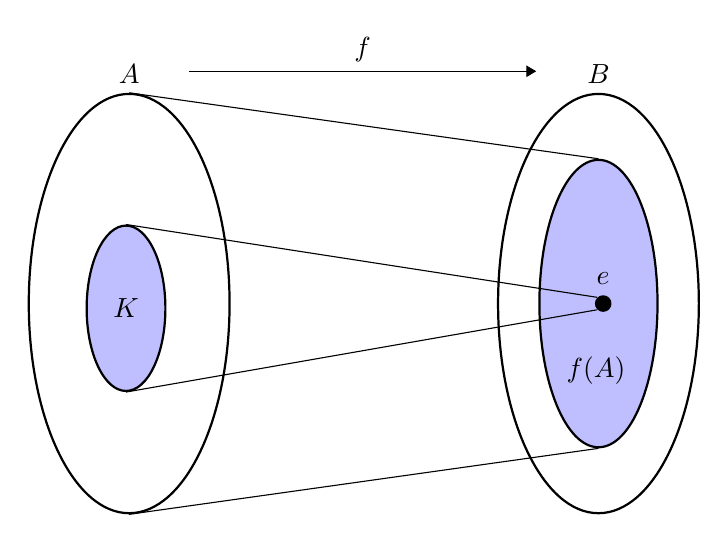
\begin{tikzpicture}
		\node[ellipse,draw,thick,minimum width=2.55cm,minimum height=5.325cm,inner sep=0pt,label={above:$A$}] (1) at (-2.83,-0.65) {};
		\node[ellipse,draw,thick,minimum width=2.55cm,minimum height=5.325cm,inner sep=0pt,label={above:$B$}] (2) at (3.13,-0.65) {};
		\node[ellipse,draw,thick,minimum width=1cm,minimum height=2.1cm,inner sep=0pt,fill=blue!25] (3) at (-2.87,-0.71) {$K$};
		\node[ellipse,draw,thick,minimum width=1.5cm,minimum height=3.65cm,inner sep=0pt,fill=blue!25] (4) at (3.13,-0.65) {};
		\node[circle,fill=black,inner sep=0pt,minimum size=6pt,label={above:$e$}](5) at (3.19,-0.65) {};
		\node at (3.1,-1.5) {$f(A)$};
		\draw (1.north) -- (4.north);
		\draw (1.south) -- (4.south);
		\draw (3.north) -- (5.north west);
		\draw (3.south) -- (5.south west);
		\node at (3.1,-1.5) {};
		\draw[-Triangle] (-2.07,2.3) -- (2.34,2.3) node[above,midway] {$f$};
	\end{tikzpicture}
\end{document}